\documentclass[10pt,twocolumn,letterpaper]{article}
\usepackage{cvpr}
\usepackage{fontspec}
\setmainfont{texgyretermes-regular.otf}[BoldFont=texgyretermes-bold.otf,ItalicFont=texgyretermes-italic.otf,BoldItalicFont=texgyretermes-bolditalic.otf]
\usepackage{graphicx,amsmath,amssymb,booktabs}
\usepackage[breaklinks,colorlinks,citecolor=blue,linkcolor=blue,urlcolor=blue]{hyperref}
\def\cvprPaperID{Course Project 2}
\def\confName{AIAA3201}\def\confYear{2027}
\title{Few-Shot Industrial Anomaly Detection on Six VisA Categories:\\Accuracy, Calibration, and Memory Reduction}
\author{Project Contributors}
\hypersetup{pdfauthor={Project Contributors},pdftitle={Few-Shot Industrial Anomaly Detection}}
\begin{document}
\maketitle
\begingroup\renewcommand\thefootnote{}\footnotetext{Anonymous public coursework release. No arXiv identifier has been assigned.}\endgroup
\begin{abstract}
We evaluate few-shot industrial anomaly detection under a shared, resource-constrained protocol on six required VisA categories. A frozen DINOv2 patch detector is compared with aligned template differences and a compact reconstruction autoencoder. The reference budget varies over 1, 2, 4, and 8 normal images with three independent reference draws. An additional, disjoint set of 40 normal images per category calibrates operating thresholds without test labels. At eight shots, the full patch memory achieves a macro image AUROC of 0.9277. Uniformly retaining one quarter of memory features reduces the bank from 24 to 6 MiB and matching-plus-map time from approximately 149 to 41 ms, with image AUROC decreasing to 0.9208. Spatial pooling at the same memory budget gives 0.8880, demonstrating a less favorable tradeoff in this setting.  A coverage-based coreset at the same 6 MiB budget obtains image AUROC 0.9294; its benefits and costs are evaluated using reference coverage and paired decision errors. The report includes pixel metrics, operating-point errors, and 24 inspected failure examples. These experiments support a practical classroom prototype rather than a claim of state-of-the-art performance. Code: \url{https://github.com/YichangLIU0/AIAA3201-Project2-AnomalyDetection}.
\end{abstract}
\section{Introduction}
Industrial inspection must distinguish a defective item from normal variation in appearance. With only a few normal reference images, the reference set may not cover object orientation, arrangement, surface texture, or illumination. A detector can therefore respond strongly to an unfamiliar normal boundary while missing a small defect. This project studies that problem using the six categories specified by the course: candle, capsules, cashew, chewinggum, fryum, and pipe\_fryum.

The experimental question has two parts. First, how do simple appearance and reconstruction baselines compare with frozen pretrained patch features under a common data split? Second, how much memory can be removed before detection and localization deteriorate? The comparison emphasizes reproducible reference sampling and a threshold chosen entirely from normal calibration data. A ranking metric alone does not establish useful OK/NG decisions.

We provide an auditable implementation, compare three quarter-size memory variants, and report the loss from pooling. Numerical experimental results are measured locally, not copied from published papers.
\section{Related Work}
MVTec AD established a benchmark for unsupervised industrial anomaly detection with normal training images and pixel annotations for evaluation~\cite{mvtec}. VisA provides the data used here~\cite{visa}. Their category distributions differ, so published MVTec performance is not a direct baseline for this VisA experiment.

PaDiM models distributions of pretrained patch representations~\cite{padim}; PatchCore uses a memory of nominal patch features~\cite{patchcore}. These approaches motivate local feature comparisons but are not reproduced in this project. Random sampling is a budget control; our projected greedy coreset borrows PatchCore's coverage objective, but is not a reproduction of its complete detector.

DRAEM combines reconstruction with discriminative learning~\cite{draem}, whereas CutPaste uses synthetic transformations for self-supervised anomaly representation learning~\cite{cutpaste}. Our plain reconstruction autoencoder does not implement either method and should not be interpreted as their measured performance.
\clearpage
\section{Data and Evaluation Protocol}
\subsection{Dataset and reference sampling}
We use the official VisA one-class split produced by the released preparation script. All test images in the six required categories are evaluated: 200 candle images, 160 capsules images, and 150 images in each remaining category, totaling 960. Test masks are used exclusively for evaluation and failure inspection. All images are resized to $224\times224$ with bicubic interpolation; masks use nearest-neighbor interpolation. This resolution reduces computational cost, but can hide very small defects and changes the localization task relative to native resolution.

For each category, a fixed random permutation with seed 20261024 reserves 40 normal training images for calibration. These images are excluded from every reference bank and autoencoder training set. For each of seeds 0, 1, and 2, eight images are sampled without replacement from the remaining pool. The 1-, 2-, and 4-shot reference sets are prefixes of the corresponding eight-image draw. Thus budgets are paired within a seed. Seeds may share references with one another; they are not disjoint datasets.

This is a few-reference protocol with extra calibration data, not a strict $K$-total-normal-image protocol. The distinction matters: even the one-shot detector uses 40 additional normal images to set a decision threshold. Image and pixel ranking metrics are threshold-independent, while FPR and FNR describe this particular calibrated operating point. Manifests record every reference, calibration image, and test path.
\subsection{Image and pixel metrics}
We report image AUROC and average precision (AP), pixel AUROC and AP, and area under the per-region overlap curve (AUPRO). Pixel metrics are evaluated on the resized masks. An image is anomalous when its mask contains any positive pixel; an audit checks this against the official good/bad folder label.

For AUPRO, each four-connected ground-truth region receives equal weight. At a score threshold, region overlap is the fraction of that region predicted positive; the mean is plotted against the fraction of all background pixels predicted positive. We integrate only up to background FPR 0.3, interpolate at that boundary, and divide by 0.3. Background pixels include those from defect-free images. This explicitly stated implementation avoids treating differently normalized AUPRO values as interchangeable.

AP complements pixel AUROC because the defect area may occupy a small fraction of an image. We do not infer good localization from a high pixel AUROC alone. All categories have equal weight in the reported macro average. For each seed we average over the six categories, then report the mean and sample standard deviation over the three seed-level macro averages. This measures reference-selection variation, not uncertainty over a population of industrial products.
\subsection{Threshold calibration}
Let $c_{(1)}\leq\cdots\leq c_{(n)}$ be the sorted normal calibration scores, with $n=40$ and target $\alpha=0.05$. The image threshold is
\begin{equation}
 \tau=c_{(\lceil(n+1)(1-\alpha)\rceil)}=c_{(39)}.
\end{equation}
The decision is NG exactly when $s(x)>\tau$. Ties are accepted as normal. With distinct calibration scores this rejects one of the 40 calibration images; it does not guarantee a particular test FPR under distribution shift. No test-set F1 maximization is used to choose the operating point.

For display, a separate pixel threshold is the 99.5th percentile of calibration-map pixel scores. This is a pooled normal-pixel quantile, not a calibrated guarantee for every image or connected component. Image OK/NG decisions use the image threshold, not the area of the thresholded display mask.
\subsection{Remaining related approaches}
DINOv2 supplies the self-supervised visual features~\cite{dinov2}. AnomalyDINO applies these features to few-shot patch matching~\cite{anomalydino}. AnomalyCLIP learns object-agnostic normal/abnormal prompts using auxiliary data~\cite{anomalyclip}; our separate comparison uses released weights rather than target-category prompt training. EfficientAD is relevant to latency-oriented inspection~\cite{efficientad}, but its published latency cannot be transferred to this laptop. The challenging acquisition settings in MVTec AD 2 motivate testing beyond clean benchmark images~\cite{mvtec2}; we do not evaluate on that dataset.
\clearpage
\section{Methods and Controlled Ablations}
\subsection{Aligned template differences}
For each eight-image reference set, we create eight rotations per reference at increments of $45^\circ$. A test image is compared against the resulting 64 templates using mean squared RGB difference at $28\times28$ resolution to select a candidate. We then estimate a Euclidean alignment with OpenCV ECC, using up to 40 iterations and a $10^{-4}$ convergence criterion. A failed alignment falls back to the unaligned template, and failures are recorded.

The anomaly map is the mean absolute RGB residual, scaled by 255 and Gaussian-smoothed with $\sigma=2$. The image score is the mean of its largest one percent of pixel values. This baseline is inexpensive, but assumes that a normal reference can be aligned meaningfully with the query. Layout changes and multiple independently oriented objects can violate this assumption even if all items are normal.
\subsection{Compact reconstruction autoencoder}
The normal-only autoencoder uses three stride-two convolutional layers with 16, 32, and 64 channels, followed by three transposed-convolution layers and a sigmoid output. It is trained from scratch with MSE loss, Adam at learning rate 0.001, batch size 8, and 15 fixed epochs. Its training set is the same 64 rotated reference images. No anomalous example is used for optimization or stopping.

The map is the smoothed mean absolute reconstruction residual and the image score again averages its largest one percent of pixels. Initialization and training order follow the reference seed. This is a deliberately compact baseline with a fixed training budget. Low performance may reflect insufficient representation or training; it does not establish that reconstruction-based methods generally fail.
\subsection{Frozen DINO patch detector}
We load the official DINOv2 ViT-S/14 pretrained weights and use the official AnomalyDINO feature and background-mask routines. At input resolution 224, each image produces a $16\times16$ grid of 384-dimensional patch features. The backbone is frozen and inference uses FP32. Each reference contributes eight rotated views. Query features use the official PCA-based background mask; an empty mask falls back to retaining every patch.

Reference and query features are $\ell_2$ normalized. FAISS performs exact nearest-neighbor search on the CPU. Since normalized vectors satisfy $\|u-v\|_2^2=2-2u^Tv$, half the returned squared distance is the cosine-distance anomaly score. Excluded background query locations receive zero score. The image score averages the highest one percent of patch scores, with at least one patch retained. Patch scores are interpolated to $224\times224$ and Gaussian-smoothed with $\sigma=4$ for pixel evaluation.

We adapt data loading, random reference selection, caching, metrics, and normal-only threshold calibration. This is a resource-constrained adaptation, not an exact reproduction of the paper's full protocol. In particular, upstream filename slicing is replaced by explicit random draws and the evaluation resolution is fixed at 224.
\subsection{Quarter-size memory variants}
At eight shots, the full bank contains $8\times8\times256=16384$ feature vectors, or 24 MiB in float32. We evaluate three variants with 4096 vectors and 6 MiB per category:
\begin{itemize}
\item \textbf{Random25}: sample one quarter of the full vectors without replacement, with a deterministic seed derived from the reference seed. The original local feature vectors are retained.
\item \textbf{Pooled25}: average each non-overlapping $2\times2$ spatial group within a reference feature map, then normalize the resulting vector. Every rotated reference contributes a coarser $8\times8$ grid.
\item \textbf{Coreset25}: retain original vectors selected by projected greedy coverage; the algorithm and diagnosis are detailed in Section~\ref{sec:coverage}.
\end{itemize}
The same reference images, query features, calibration images, test images, distance computation, and score aggregation are used. All compressed variants therefore have the same bank size. Pooling changes representation as well as count, whereas random sampling only changes which original features are kept. The comparison tests representation averaging and coverage-based selection at the same budget; it does not establish optimal compression.
\begin{figure}[h]
\centering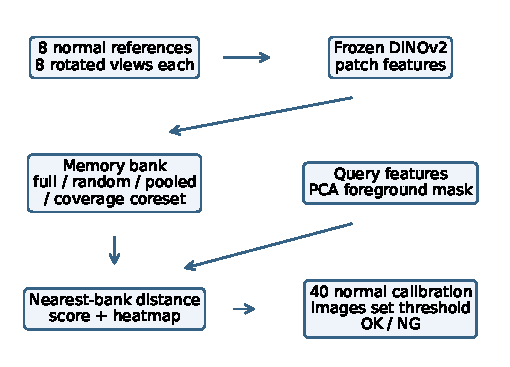
\includegraphics[width=\linewidth]{figures/pipeline.pdf}
\caption{Shared frozen-feature pipeline. Only bank construction changes; reference draws, query processing, calibration and evaluation stay fixed.}
\end{figure}
\clearpage
\section{Quantitative Results}
\begin{table*}[t]\centering\small
\caption{Macro mean $\pm$ sample standard deviation over three reference seeds. CLIP has one fixed evaluation (no seed deviation). All methods use 40 additional calibration normals per class. Metrics range from 0 to 1; lower FPR/FNR is better.}
\resizebox{\textwidth}{!}{\begin{tabular}{lrccccccc}\toprule
Method & Shots & I-AUROC & I-AP & P-AUROC & P-AP & AUPRO$_{.3}$ & FPR & FNR \\ \midrule
AnomalyCLIP & 0 & 0.842 & 0.906 & 0.960 & 0.245 & 0.847 & 0.034 & 0.470 \\
Autoencoder & 8 & $0.621\pm0.034$ & $0.748\pm0.020$ & $0.782\pm0.022$ & $0.056\pm0.003$ & $0.545\pm0.030$ & $0.049\pm0.011$ & $0.792\pm0.039$ \\
DINO coreset25 & 8 & $0.929\pm0.003$ & $0.960\pm0.002$ & $0.981\pm0.000$ & $0.427\pm0.009$ & $0.883\pm0.006$ & $0.042\pm0.009$ & $0.303\pm0.032$ \\
DINO full & 1 & $0.903\pm0.009$ & $0.942\pm0.008$ & $0.975\pm0.001$ & $0.386\pm0.023$ & $0.867\pm0.002$ & $0.037\pm0.015$ & $0.373\pm0.022$ \\
DINO full & 2 & $0.916\pm0.012$ & $0.952\pm0.006$ & $0.978\pm0.001$ & $0.398\pm0.013$ & $0.873\pm0.003$ & $0.036\pm0.015$ & $0.323\pm0.030$ \\
DINO full & 4 & $0.919\pm0.004$ & $0.954\pm0.003$ & $0.980\pm0.001$ & $0.418\pm0.008$ & $0.877\pm0.003$ & $0.028\pm0.020$ & $0.308\pm0.035$ \\
DINO full & 8 & $0.928\pm0.003$ & $0.959\pm0.002$ & $0.981\pm0.000$ & $0.427\pm0.008$ & $0.879\pm0.003$ & $0.048\pm0.004$ & $0.274\pm0.011$ \\
DINO pooled25 & 8 & $0.888\pm0.001$ & $0.936\pm0.001$ & $0.969\pm0.001$ & $0.373\pm0.005$ & $0.858\pm0.003$ & $0.034\pm0.013$ & $0.376\pm0.055$ \\
DINO random25 & 8 & $0.921\pm0.003$ & $0.954\pm0.001$ & $0.978\pm0.001$ & $0.412\pm0.002$ & $0.872\pm0.004$ & $0.051\pm0.022$ & $0.288\pm0.023$ \\
Template ECC & 8 & $0.663\pm0.017$ & $0.776\pm0.007$ & $0.816\pm0.005$ & $0.180\pm0.005$ & $0.509\pm0.004$ & $0.049\pm0.012$ & $0.813\pm0.009$ \\
\bottomrule\end{tabular}}\label{tab:main}\end{table*}
\subsection{Baseline comparison}
Template ECC reaches macro image AUROC 0.663, and the compact autoencoder reaches 0.621. The fixed AnomalyCLIP checkpoint obtains 0.842, compared with 0.928 for eight-shot full-memory DINO. These are measured results under the present 224-resolution adaptation, not the published performance of these methods. The gap cannot be attributed solely to model architecture because pretrained data, model size, and target fitting differ.

\subsection{Effect of reference budget}
Increasing the number of normal references improves aggregate ranking in this experiment. Image AUROC rises from approximately 0.903 at one shot to 0.928 at eight shots. Pixel AP and AUPRO also improve on average. These aggregate trends do not imply monotonic gains for every category or every sampled reference set. The plotted error bars show variation across reference draws for a fixed benchmark.
\begin{figure*}[t]
\centering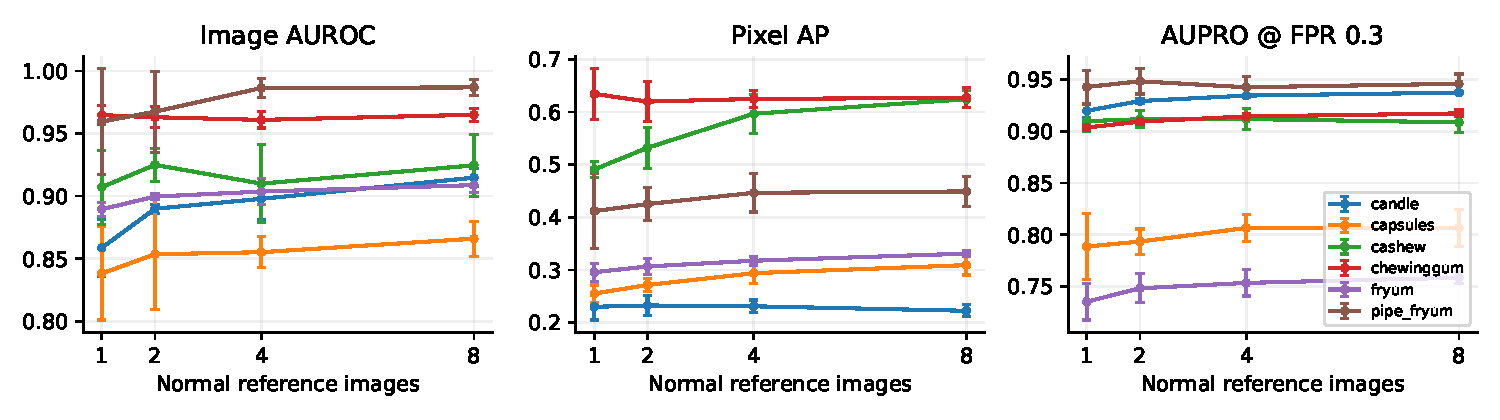
\includegraphics[width=.95\textwidth]{figures/shot_curves.pdf}
\caption{Full-memory DINO detector across reference budgets. Curves are category means over three draws; error bars are sample standard deviations. The same seeded draw is nested across shot counts.}
\end{figure*}
\subsection{Compression tradeoff}
Random25 retains most of the measured ranking performance at one quarter of the memory. The mean matching-plus-map time drops by about 3.6 times, but this excludes feature extraction, image decoding, and application overhead. It is therefore not a claim of a 3.6-times end-to-end speedup.

Pooled25 gives lower image AUROC than Random25 at the same bank size. A plausible explanation is that averaging neighboring features blends normal structures whose distinct representations are useful for matching. The ablation supports the performance difference, but does not isolate that mechanism causally. No alternate pooling scale or learned pooling was tuned on the test set.
\subsection{Operating point versus ranking}
The normal-calibrated threshold makes the prototype conservative about declaring defects in some categories. A strong image AUROC can coexist with substantial FNR at this operating point. Threshold adjustment for a production application would require an appropriate validation protocol and an explicit cost tradeoff; selecting a threshold that maximizes test F1 would give an optimistic estimate of deployment performance.

The baseline and pretrained comparisons share test images and calibration rules, but their pretraining resources differ. DINOv2 and the released AnomalyCLIP model encode external training information, whereas the autoencoder learns from the small target reference set. The comparison describes available approaches under these resource choices, not a controlled test of architecture alone.
\subsection{Resource measurements}
The mean DINO query-feature time is 71.9 ms, separately measured from the 149.0 ms full-memory matching and map stage. Random25 and Pooled25 matching take 41.0 and 40.0 ms respectively. Adding the measured feature component gives approximately 220.9 versus 112.9 ms for full and Random25, before image loading and application overhead. Cached component measurements are not a direct wall-clock demo benchmark.

Template ECC, autoencoder, and AnomalyCLIP inference components average 47.2, 6.6, and 193.8 ms. Inputs are loaded before these timing regions. The compact autoencoder takes 2.5 seconds to train on average under its small fixed budget. Peak allocated GPU memory is approximately 97 MiB for DINO, 53.5 MiB for the autoencoder including training, and 1692 MiB for AnomalyCLIP. These are different execution scopes; the values document resource use rather than an equal-architecture efficiency ranking. The template baseline is CPU-only.
\subsection{Bounded brightness stress test}
We additionally select the first ten good and ten bad test images by filename from each category, giving a fixed 120-image subset. RGB values are multiplied by 0.8, 1.0, or 1.2 and clipped to the valid range. Seed-0 eight-shot banks and clean calibration thresholds remain unchanged. This gives 54 category--brightness--method evaluations, separate from the 168 main runs.

For full memory, macro image AUROC is 0.947, 0.925, and 0.910 across the three factors; Random25 gives 0.947, 0.925, and 0.917. The non-monotonic response across methods and metrics cautions against a simple robustness claim. The subset is small and filename-selected, and synthetic RGB scaling is not real acquisition under different illumination. These results cannot replace the full-test metrics or demonstrate deployment robustness.

\begin{figure}[b]
\centering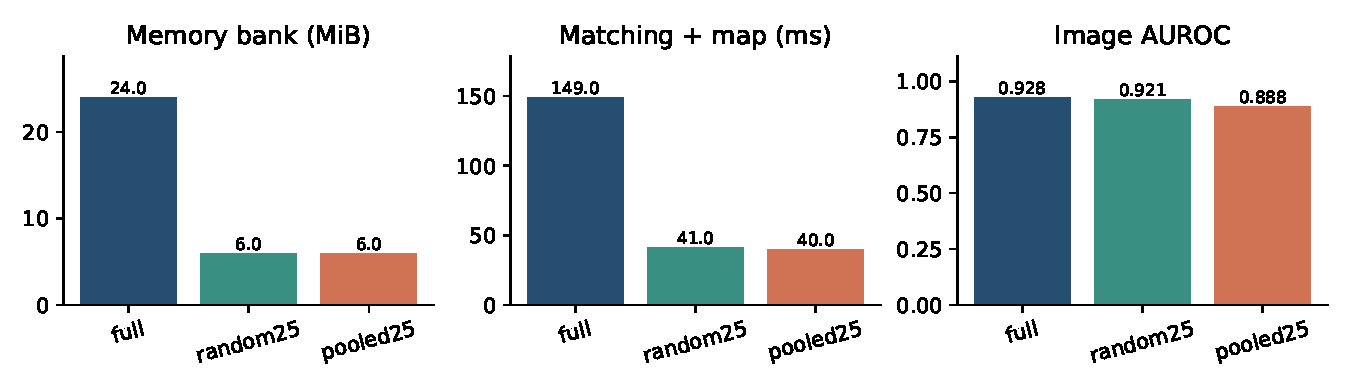
\includegraphics[width=\linewidth]{figures/compression.pdf}
\caption{Eight-shot memory, CPU matching-plus-map time, and image ranking. The timing component excludes the GPU backbone. Lower memory does not imply higher accuracy.}
\end{figure}
\clearpage
\section{Coverage-Preserving Compression}\label{sec:coverage}
\subsection{Concrete problem and proposed remedy}
Uniform random compression can discard reference features that represent less common normal appearances. This can increase the distance assigned to a legitimate query even when it has a close match in the full bank. The visible normal-boundary and texture false alarms motivate examining that possibility, but are not proof of a compression-induced cause: many already occur with full memory.

We therefore distinguish two questions: does selection preserve the original feature coverage, and does that preservation improve decisions on held-out images? These require separate measurements. Our method is a projected greedy $k$-center baseline inspired by PatchCore~\cite{patchcore}; the course contribution is the controlled diagnosis and adaptation, not invention of coreset selection.
\subsection{Fixed algorithm and evaluation}
Starting from the normalized 384-dimensional reference vectors, we apply a fixed Gaussian projection to 128 dimensions, seeded by the reference seed plus 2000. The first center is furthest from the projected mean. Each subsequent center maximizes its distance to the closest selected center. We select 4096 distinct indices and store their original 384-dimensional vectors. Selection sees neither calibration nor test labels, and no backbone weights change. Projection dimension and budget are fixed before evaluating this extension.

All three compressed methods use 6 MiB. We retain the original references, PCA query masks, distances, maps, and normal-only calibration rule. The 18 added runs cover every category and reference seed. Coverage is measured in the original feature space: for every original reference vector, find its nearest retained vector and measure cosine distance. The table reports the mean of per-run maxima, rather than a worst-case bound over unseen images.
\begin{table}[h]\centering\small
\caption{Equal-budget comparison. Coverage is mean worst reference cosine distance; lower is better. FPR/FNR are category-macro averages with each method's normal-calibrated threshold.}
\begin{tabular}{lrrrr}\toprule
Method & Coverage & AUROC & FPR & FNR\\\midrule
random25 & 0.288 & 0.921 & 0.051 & 0.288\\
pooled25 & 0.422 & 0.888 & 0.034 & 0.376\\
coreset25 & 0.111 & 0.929 & 0.042 & 0.303\\
\bottomrule\end{tabular}\end{table}
\subsection{Measured outcome and tradeoffs}
The average worst reference distance changes from 0.288 for random sampling to 0.111 for coreset selection. Image AUROC changes from 0.9208 to 0.9294, and pixel AP from 0.4118 to 0.4275. These observations must be interpreted together: optimizing reference coverage need not optimize anomaly separation.

Across the paired evaluations, coreset fixes 27 random-bank false positives and introduces 20; it fixes 50 false negatives and introduces 78. Counts refer to image--seed events, not distinct images: the same test image is evaluated under three reference draws. Both recovered and newly introduced errors are saved as explicit examples. A lower normal score alone is insufficient evidence because the calibrated threshold also changes.

Offline coreset selection averages 2.95 seconds per category/seed, versus approximately 0.029 seconds for random-bank construction. Matching plus map generation averages 29.3 ms, with the shared feature-extraction component excluded. Selection-only peak allocated GPU memory averages 40.3 MiB and is separate from the backbone allocation. This offline cost must be amortized over repeated queries. Equal-size exact-search banks have the same nominal search workload; timing differences between their separate runs are not evidence of an algorithmic speed advantage.

\subsection{What this establishes}
The extension makes the problem--method--evaluation link explicit and adds a matched strong selection baseline. It does not establish that coverage alone causes the observed errors, that coreset dominates every metric/category, or that the method is novel. The subset brightness experiment still covers only the original three banks; no coreset robustness result is implied.
\begin{figure}[h]
\centering
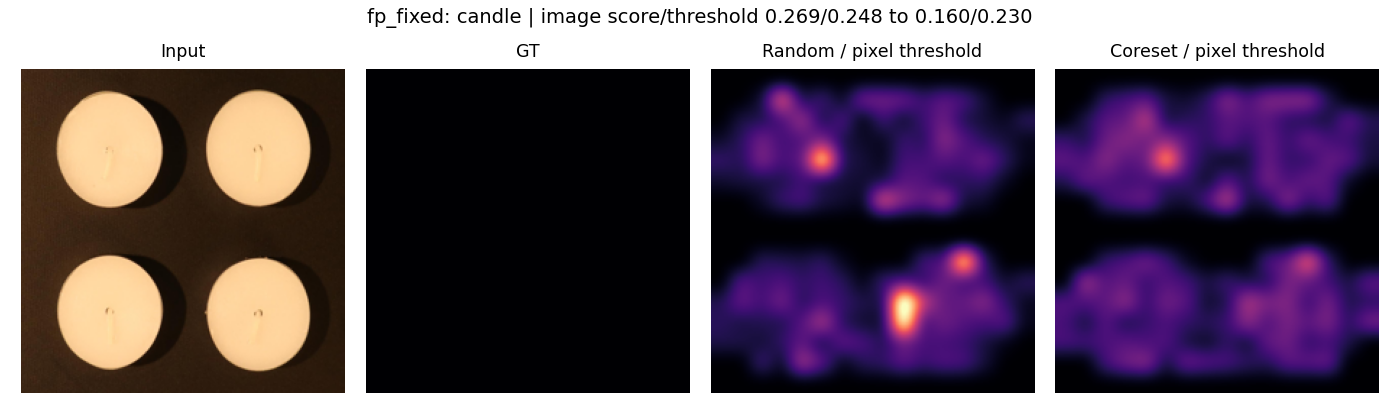
\includegraphics[width=\linewidth]{figures/coreset_fp_fixed.png}
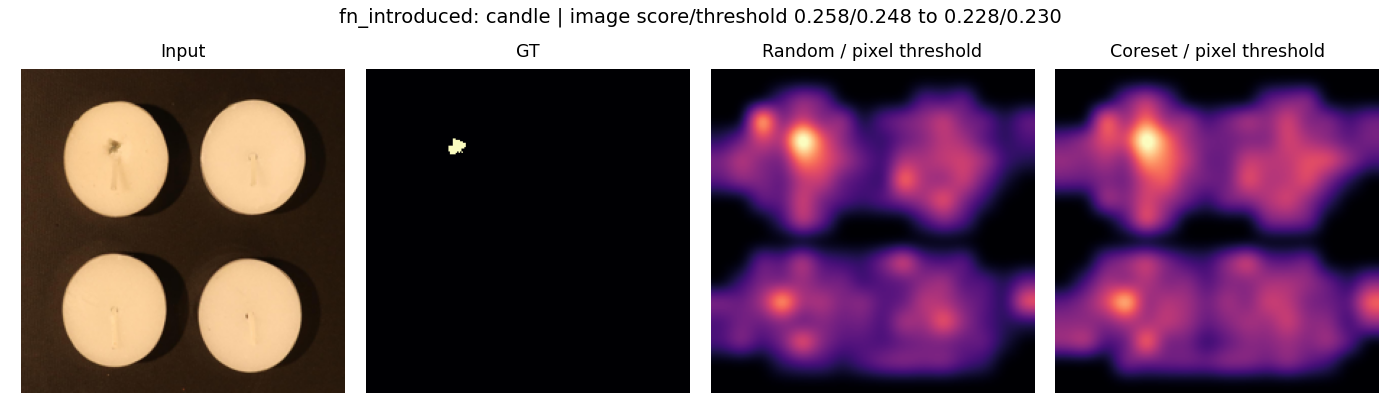
\includegraphics[width=\linewidth]{figures/coreset_fn_introduced.png}
\caption{Both sides of the tradeoff: a corrected normal-image false alarm (top) and a newly missed defect (bottom). Columns show input, GT, random-bank map and coreset map. Maps are divided by their normal-calibrated pixel thresholds; identical display range does not imply identical raw scores.}
\end{figure}
\clearpage
\section{Qualitative Results and Failure Analysis}
\begin{figure}[t]
\centering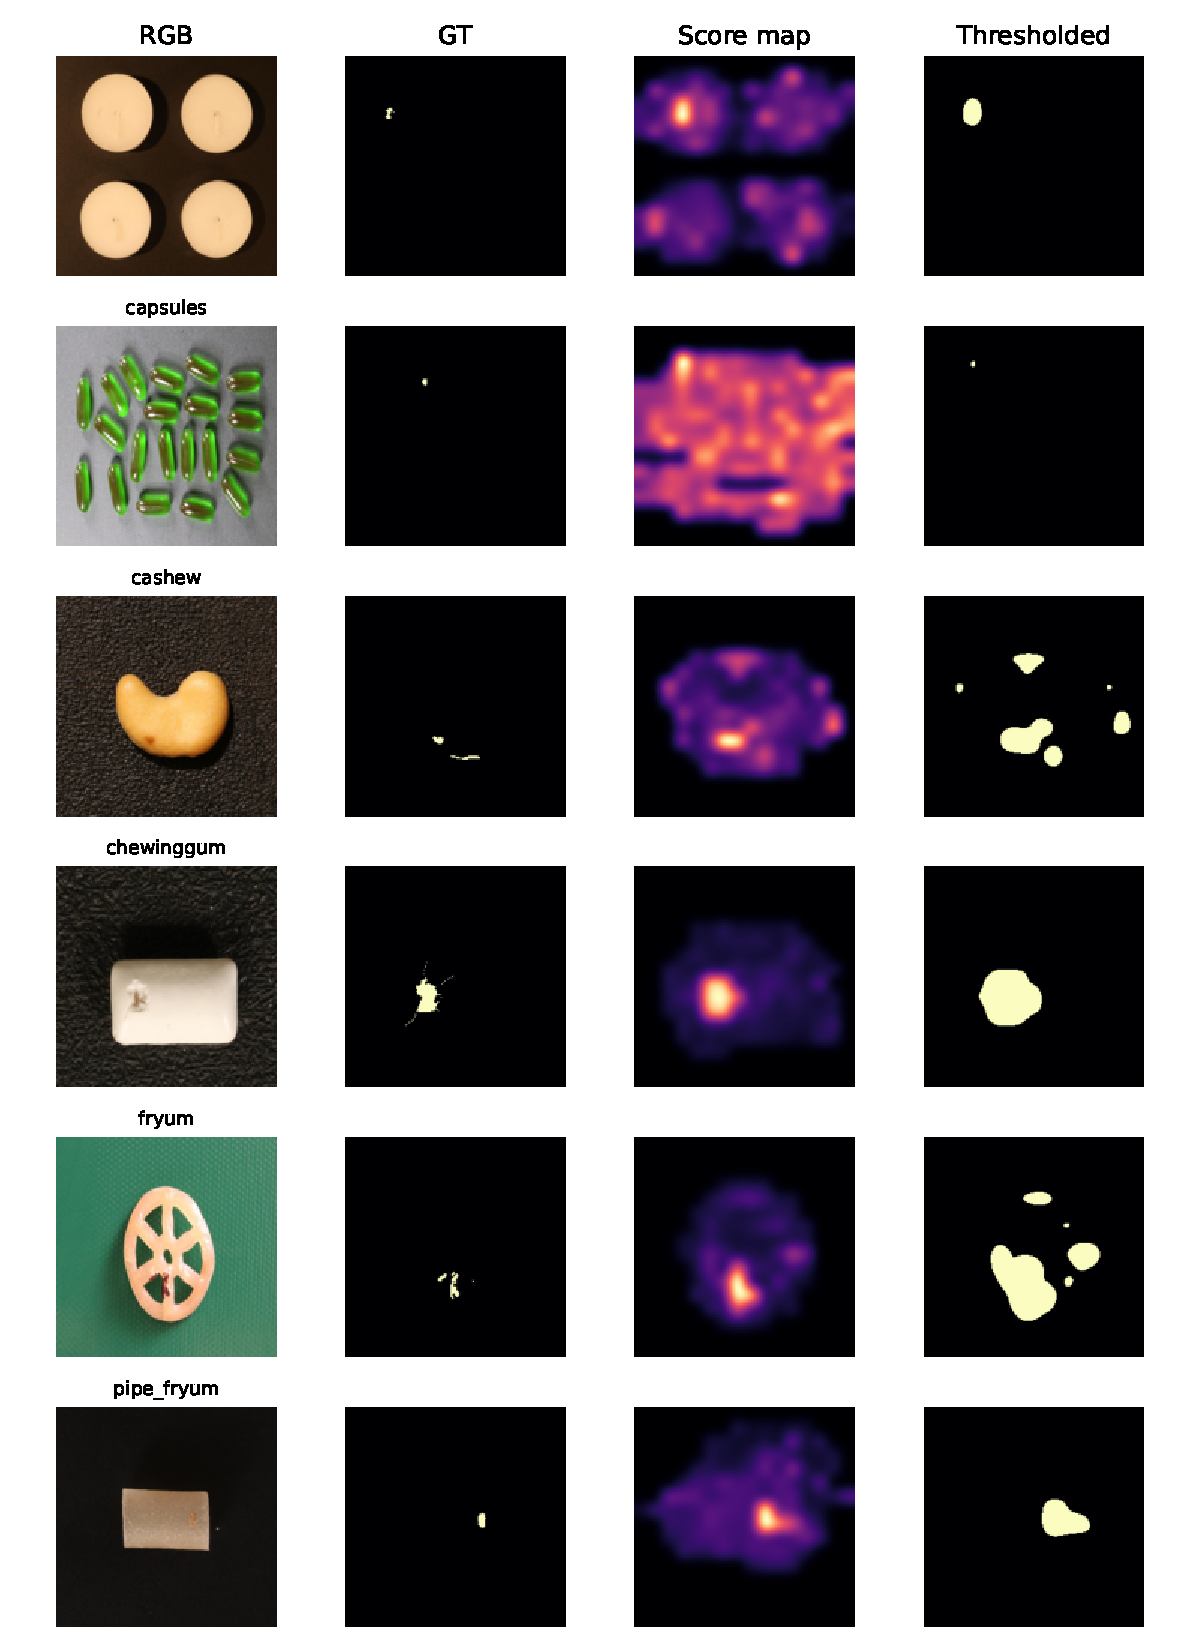
\includegraphics[width=.92\linewidth,height=.68\textheight,keepaspectratio]{figures/qualitative.pdf}
\caption{One fixed anomalous test example per category: input, ground truth, anomaly map, and thresholded map. Examples are selected by filename order, not by best performance. Heatmap intensity alone is not the image decision.}
\end{figure}
We inspected 24 errors from the full eight-shot detector with seed 0. The selection attempts two false positives and two false negatives per category, then fills any shortfall with other errors. Cashew has no selected false positives and contributes four false negatives. The resulting set contains 10 false positives and 14 false negatives. These are illustrative examples, not a random sample or an estimate of error-type prevalence. Individual paths, scores, thresholds, masks, and observations are included with the code.

\textbf{Normal boundaries and arrangement.} Candle false positives highlight intact rims and surfaces. Capsules errors include responses near image boundaries and differently oriented normal instances. Fryum false positives highlight otherwise normal rims or spokes. These observations suggest sensitivity to reference coverage and local geometry, but do not prove whether pose, lighting, or the feature representation is responsible.

\textbf{Small defects and conservative thresholds.} Several capsule, cashew, and chewinggum false negatives have localized heatmap responses that fail to cross the image threshold. Some annotated defects occupy only a small region relative to the 16-by-16 feature grid. Resolution and top-score aggregation are plausible contributors. Distinguishing their effects would require a matched-resolution and aggregation ablation.

\textbf{Background responses.} A chewinggum false positive includes a hotspot above the object, and some multi-instance examples respond strongly near the field boundary. This motivates inspecting the PCA mask rather than assuming it removes all irrelevant background. The present mask is inherited from the upstream implementation, with only an empty-mask safeguard.

\textbf{Texture versus defects.} Pipe-fryum false positives respond to normal surface texture, whereas selected false negatives include a thin boundary notch and a pale local blemish. The observations indicate overlap between benign texture variation and weak anomaly responses. A larger nominal reference set may help, but this remains a hypothesis beyond the tested budgets.

The contact sheets show both ground-truth masks and predictions so that the discussion can be checked visually. Proposed causes are explicitly separated from visible facts. In particular, a missed decision does not mean the anomaly map is completely uninformative, and a plausible-looking heatmap does not establish correct detection.
\clearpage
\section{Implementation, Demo, and Limitations}
\subsection{Hardware and reproducibility}
Experiments run on an NVIDIA RTX A500 Laptop GPU with 4 GB of memory. Feature extraction runs on the GPU, while exact FAISS matching uses four CPU threads. Reported CUDA peak allocation is PyTorch allocated memory rather than total device occupancy. Cached features reduce repeated experiment cost, but caching time is not counted as online inference latency. The artifact includes source revisions, weight and archive hashes, data manifests, configuration in source, and per-run metrics.

The virtual environment inherits camera\_sdk and is not portable. The README records fresh installation steps; datasets and weights are separate downloads.
\subsection{AnomalyCLIP comparison}
The additional comparison loads the official released target-VisA prompt checkpoint and the ViT-L/14 CLIP backbone. There is no target-category gradient update. Inputs and pixel metrics use 224 resolution, and the released script's selected feature layer is retained. The operating threshold still uses the same 40 target normal calibration images, so the complete decision pipeline is not target-data-free. A single fixed checkpoint evaluation has no reference-draw standard deviation; repeating deterministic evaluation would not create meaningful independent trials.

This model has a larger pretrained backbone and different auxiliary learning than the DINO model. Its results should therefore be interpreted as an additional practical baseline, not an equal-pretraining-capacity comparison. Resolution and calibration adaptations are documented rather than described as exact paper reproduction.
\subsection{Runnable inspection interface}
The demo loads a category-specific bank and accepts a product image. It displays the input, anomaly heatmap, overlay, calibrated pixel mask, continuous image score, threshold, and OK/NG decision. Random25 is the default because it reduces bank size with a relatively small ranking loss in this experiment. The full, pooled and coreset banks remain selectable for comparison.

The heatmap uses a category-specific scale derived from normal calibration rather than stretching each image independently. The thresholded display mask is not a segmentation guarantee. The category must be selected correctly, and an OK decision does not certify that an item is defect-free. The accompanying random and coreset demonstrations record actual predictions, including the continuous score needed to interpret decisions near the threshold.
\subsection{Limitations and next experiments}
Only six VisA categories are evaluated, at reduced resolution and with three reference draws. This does not support broad claims about industrial deployment or statistically established superiority across datasets. The compact autoencoder has a fixed 15-epoch budget; stronger reconstruction training might change its performance. Calibration uses additional normal images, which must be disclosed when comparing to stricter few-shot protocols.

The quarter-bank experiment now includes projected greedy coreset selection. It remains a comparison of existing selection principles, not evidence of a novel compression algorithm. Projection dimension and budget are fixed; we do not claim an optimal operating point. Further useful tests include higher-resolution inference with the same references, alternate score aggregation under a separate validation design, and repeated acquisition under real lighting changes. The measured synthetic brightness perturbations are a bounded stress test rather than evidence of real production robustness.

The inspected errors motivate future tests, not causal conclusions. The repository is public; arXiv deposition remains pending.
\section{Conclusion}
Under the shared six-category protocol, frozen DINO patch matching provides a reproducible few-shot detector with interpretable memory and latency costs. Quarter-size random memory retains most of the measured image ranking quality, while spatial pooling loses more accuracy at the same memory size. The matched coreset extension explicitly tests reference coverage against detection outcomes and records both corrected and introduced errors. Normal-only calibration exposes misses that ranking metrics alone conceal. The resulting project delivers measured comparisons and an inspection prototype, with explicit limits on resolution, calibration data, pretraining fairness, and generalization.
\paragraph{Attribution and assistance.} Upstream implementations and pretrained weights are credited in the source documentation. AI assistance was used for coding, experiment orchestration, and manuscript preparation. Contributors should confirm course submission and disclosure requirements.
\clearpage
{\small\bibliographystyle{ieeenat_fullname}\bibliography{references}}
\end{document}
